\section{Results}
Things to show:
\begin{enumerate}
    \item Introduce datasets and metric(s)
    \begin{enumerate}
        \item Artificial dataset that breaks uniform sampling
        \item Benchmark dataset from ESA paper
        \item Geometric dataset that breaks lightweight coresets
    \end{enumerate}
    \item Running sensitivity sampling with kmeans++ does not scale with $k$ but fast-kmeans++ solution does
    \item Uniform sampling and lightweight coresets both don't work on simple toy datasets
    \item The size of the coreset seems to make a difference when performing sensitivity sampling but not as much
          when doing lightweight coreset and uniform
\end{enumerate}

\subsection{Experimental Setup}
\subsubsection{Metrics}

We analyze the coreset construction methods along two metrics -- quality and construction time.  Although measuring runtime is standard, predicting coreset
quality is a more difficult task. Specifically, it is unclear how to confirm that a subset of points satisfies the coreset property over all solutions. To this
end, the authors in \cite{chrisESA} suggested reporting the following metric 
\[ \max \left( \dfrac{\cost(P, \calC_{\Omega})}{\cost(\Omega, \calC_{\Omega})}, \dfrac{\cost(\Omega, \calC_{\Omega})}{\cost(P, \calC_{\Omega})} \right),\]
where $\calC_{\Omega}$ is a candidate solution that was computed over the coreset.

We refer to this metric as the \emph{coreset distortion}. Naturally, values that are consistently close to $1$ suggest that solutions on the coreset are likely
viable on the full dataset.

\begin{figure*}
\label{fig:lightweight_breaks}
\centering
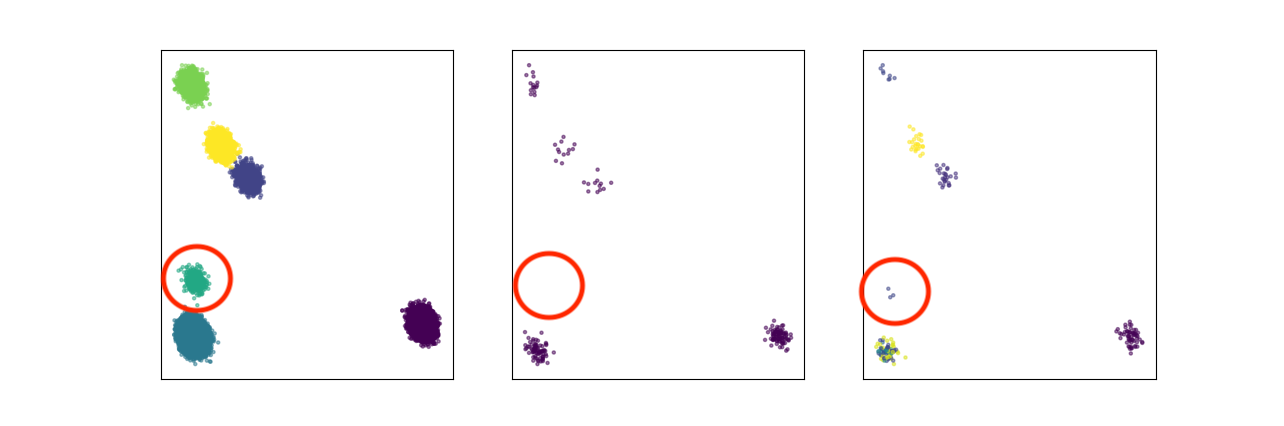
\includegraphics[width=.95\linewidth]{images/lightweight_breaks.png}
\caption{
The results of lightweight and fast-coreset constructions on a dataset of $n=100K$ points with clusters of varying size. Coresets have 200 points.
\emph{Left}: Original multivariate-Gaussian dataset. \emph{Middle}: Lightweight coresets fail to capture the cluster of $\sim$400 points.
\emph{Right}: The Fast-coreset construction runs in linear time but identifies all of the clusters.
}
\end{figure*}

\david{the lightweight corereset is also linear time, I removed the comment about running time of fast coreset. We need to reference somewhere this figure}

\subsubsection{Algorithms}
\david{Maybe bullet points to list the algorithms, with names for the algorithm? The algorithm using $j$-means does not formally have one and is referred to in different ways afterwards}

We analyze six different algorithms for constructing coresets.
\begin{itemize}
        \item \emph{Standard uniform sampling}: choose a subset of $m \ll n$ points uniformly from $P$.
        \item \emph{Lightweight coreset}: find the mean $\mu$ of the dataset and obtain per-point sensitivity estimates by $\hat{s}(p) = 1/|P| + \cost(p, \mu) / \cost(P, \mu)$.
            The first term encourages uniform sampling while the second encourages sampling proportionate to the distance from the mean.
        \item \emph{Birch using Coresets (BICO)}: use BIRCH algorithm~\cite{birch} to create streaming coreset quickly.
        \item \emph{$j$-means++ coreset}: find an approximate $j$-means solution with $j = f(k)$ with $0 < f(k) < k$ for all $k$. We will sometimes use the notation
            $f(k)$-means++ coreset when discussing a coreset built with respect to a specific function of $k$. For example, the $\log k$-means++ solution.
        \item \emph{Standard sensitivity sampling}: obtain an approximate $k$-means solution with $k$-means++ and sample coreset proportionate to sensitivity upper bounds.
        \item \emph{Fast-Coreset}: obtain an approximate $k$-means solution with \fkmeans and sample coreset proportionate to sensitivity upper bounds.

\end{itemize}

We take a moment here to motivate the $j$-means coreset algorithm.  Consider that lightweight coresets are simply solving $1$-means to obtain sensitivity values
whereas sensitivity sampling is solving the $k$-means problem.  As we will show, it is easy to construct examples where lightweight coresets fail to produce
acceptable coresets while sensitivity-sampling produces satisfactory coresets across datasets and settings. Thus, we study the $j$-means coreset
algorithm to answer the following question: for which values of $j < k$ does an approximate $j$-means solution give a satisfactory coreset?

\subsubsection{Datasets}
\begin{figure}
\centering
\begin{tabular}{lc}
    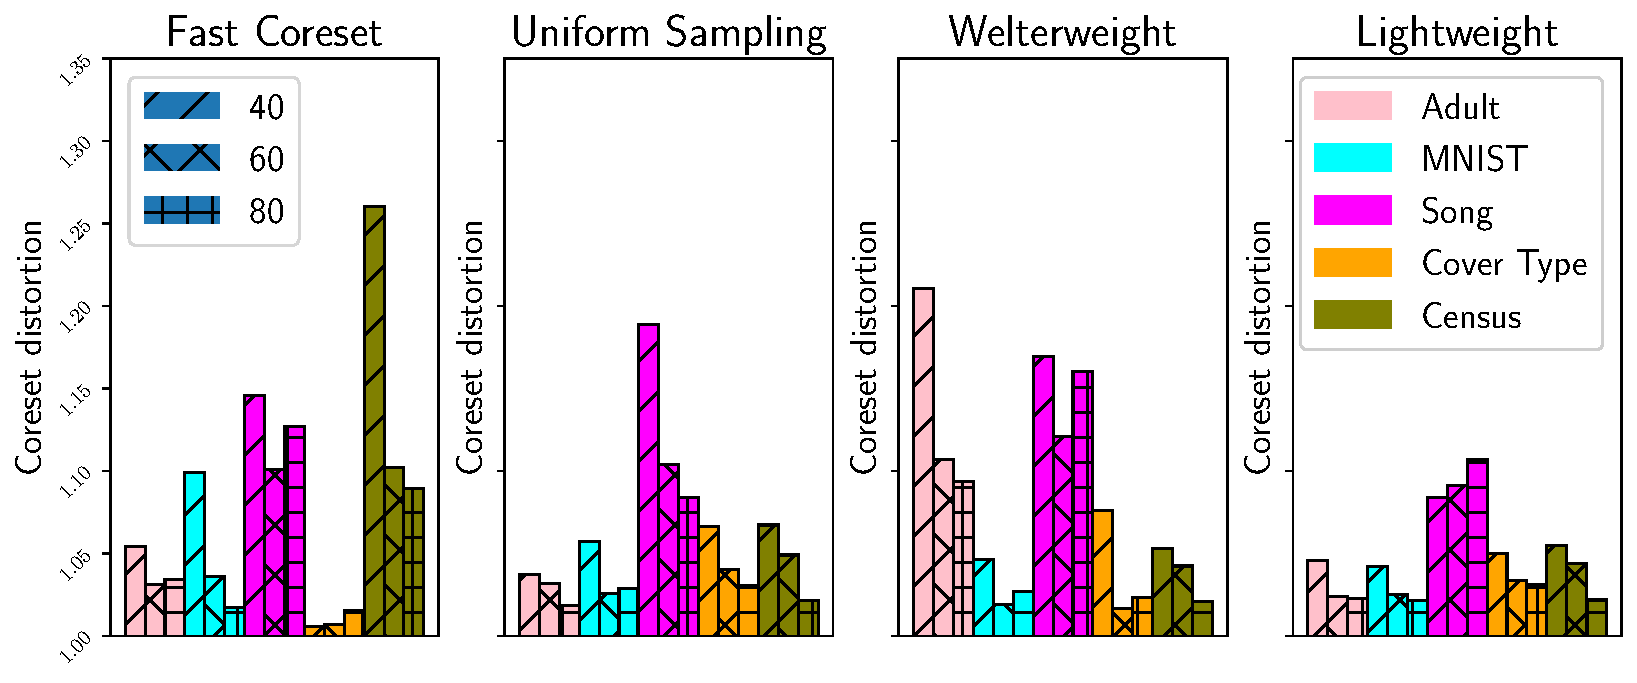
\includegraphics[width=\linewidth]{images/distortion_real_data} \\
    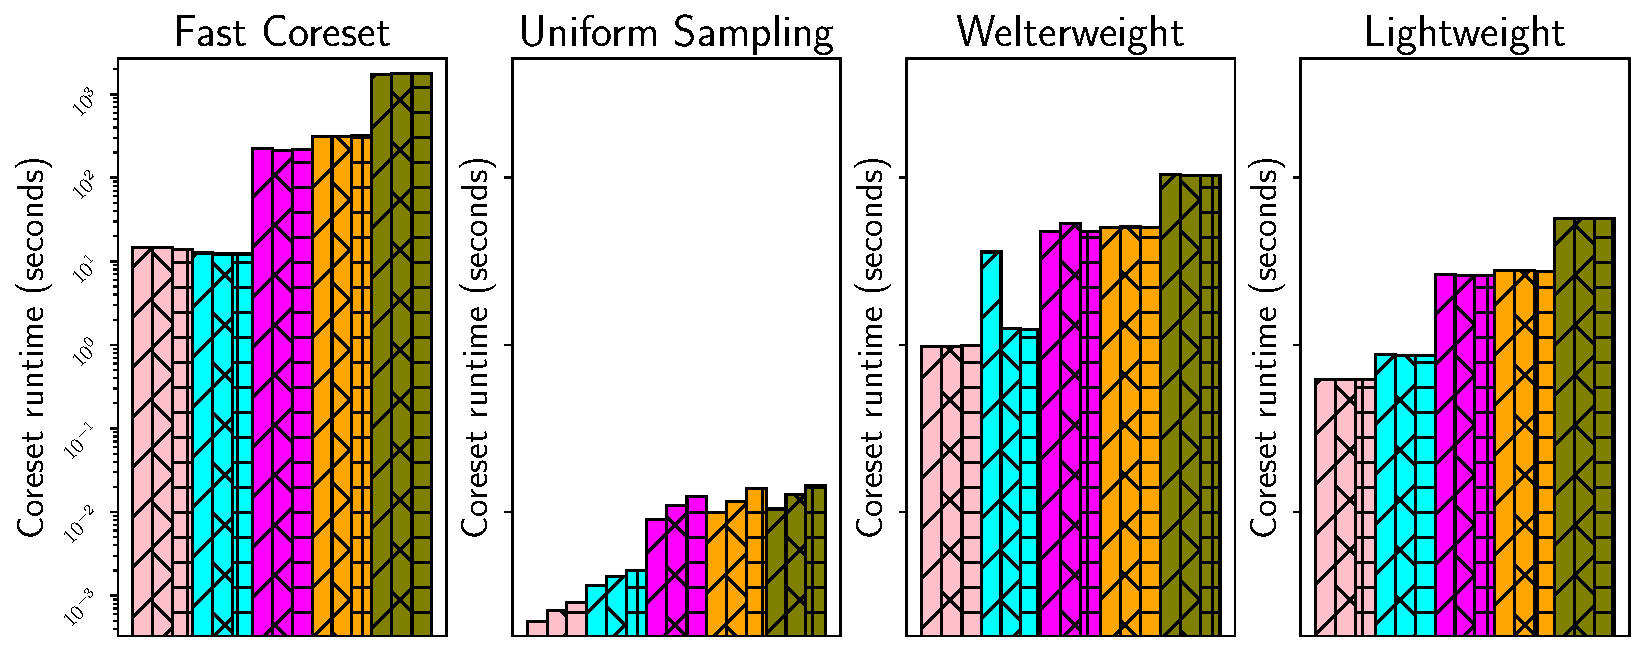
\includegraphics[width=\linewidth]{images/runtime_real_data}
\end{tabular}

\caption{\emph{Top}: The effect of the $m$-scalar on coreset distortion for real-world datasets. This is a visualization of the data in
Table~\ref{tbl:distortion}.  \emph{Bottom}: The effect of the $m$-scalar on the algorithm runtime for real-world datasets. All values are the mean over 5 runs.
The three bars represent samples of size $m=40k, 60k, 80k$.}

\label{fig:coreset_size_on_quality}
\end{figure}


We employ several real and artificial datasets to evaluate the quality of a coreset. We define the artificial datasets below and refer the reader to
Table~\cref{tbl:datasets} for the real datasets.

\begin{itemize}
    \item \emph{c-outlier}: $n-c$ points in a single location and $c$ points placed at a large distance away.
    \item \emph{Gaussian mixture}: multivariate Gaussians with varying cardinalities arranged randomly in high-dimensional space.
    \item \emph{Geometric}: $n/2$ points at $(c, 0, 0, \cdots)$, $n/4$ points at $(0, c, 0, \cdots)$, and so on.
    \item \emph{Benchmark}: A specific distribution of points such that all reasonable solutions are of equal quality but are maximally far
            apart in the solution space, as defined in \cite{chrisESA}.
\end{itemize}

\begin{table}[htbp]
    \label{tbl:datasets}
    \centering
    \begin{tabular}{lrr}
        Dataset & Points & Dim \\
        \hline
        \emph{MNIST} & 60\,000 & 784 \\
        \emph{Song} & 515\,345 & 90 \\
        \emph{Cover Type} & 581\,012 & 54 \\
        \emph{Census} & 2\,458\,285 & 68
    \end{tabular}
    \caption{Description of real world datasets}
\end{table}

For our real-world data, we utilize the MNIST~\cite{mnist}, Song~\cite{song}, Census~\cite{census}, and Cover Type~\cite{covtype} datasets. In
all real and artificial datasets, we add random uniform noise $\eta$ with $0 \leq \eta_i \leq 0.001$ in each dimension in order to make all points unique.

\subsection{Algorithm Comparisons}
\label{ssec:alg_qualities}

We first verify the fact that coreset quality is independent of whether we used $k$-means++ or \fkmeans to obtain the preliminary solution. To this end,
Figure~\ref{fig:coreset_size_on_sens_quality} shows that, across datasets, the Fast-Coreset method produces coresets of consistent quality, with all distortion
values being lower than $1.2$. Additionally, for sufficient coreset sizes ($m \approx 80\cdot k$), Fast-Coresets obtain similar distortion to those obtained
through sensitivity sampling. Despite this, Figure~\ref{fig:k_on_runtime} confirms that, while traditional sensitivity sampling runtimes grow linearly with $k$,
Fast-Coreset only grow logarithmically with the number of centers.  Therefore, our experimental findings confirm the theory predicted by \cref{thm:main}:
sensitivity sampling coresets can be implemented in linear time while preserving the coreset property. Given this context, we will not add traditional
sensitivity sampling to further experiments, as it is too slow to run on our large datasets and does not provide better quality results than the Fast-Coreset
method.

We now refer the reader to Figure~\ref{fig:coreset_size_on_quality}, where we show the effect of coreset size on the distortion across datasets and methods.  We
define the coreset sizes as $|\Omega| = ck$, where $c \in [20, 40, 60, 80]$. We see that, across datasets, coresets of larger size obtain lower distortion.
However, it is also clear that uniform, lightweight, and $j$-means coresets all fail on the geometric-progression and Gaussian-mixture datasets. Additionally,
uniform sampling expectedly fails on the $1$-outlier problem.

As discussed, the sensitivities for lightweight coresets are obtained by a linear combination of a uniform distribution and each point's relative
distance to the mean. Since the Gaussian mixture dataset has randomly distributed clusters of varying sizes, a small cluster that is close to the mean is unlikely
to ever be sampled. We argue that, although this is a toy dataset, one can easily imagine many datasets that have this property. As a simple solution, we see
that the $j$-means coreset obtains satisfactory solutions on the Gaussian mixture dataset for 

A similar argument can be made for the more-challenging geometric dataset, where the cluster size decreases exponentially and all clusters are equidistant.
We show furthermore that, for small values of $j$, sensitivities obtained according to
solving the $j$-means problem are insufficient to create a coreset for the geometric-progression dataset.

To measure the effect that the class imbalance has on the quality of each coreset, we define a class imbalance parameter $\gamma$ and obtain each
cluster's size by $|C_i| = \frac{n}{m} \exp \left( \gamma(\rho - \frac{1}{2}) \right)$, where $\rho$ is distributed uniformly at random in the range $[0, 1]$.
Thus, each cluster has size $\frac{n}{m}$ when $\gamma = 0$ and the cluster size diverges exponentially as $\gamma$ grows linearly. We see the effect of $\gamma$ on the coreset
distortion in Table \textcolor{red}{Table ref}, where even small values of $\gamma$ can break the lightweight coreset construction. Looking at the
$j$-sensitivities, we see that using $(j=\sqrt(k))$-means++ solutions maintains the coreset property for higher values of $\gamma$ but is still not guaranteed
to obtain satisfactory coresets. Despite this, sensitivity sampling consistently obtains coresets with low distortion.

As a harder example, we provide a \emph{geometric-progression} dataset, consisting of \david{Are they precisely at $(c, 0, 0, \cdots)$ or very close? if they are precisely there, scaling $c$ should not change. Maybe say $c=1$ and a tiny
noise?}. 
Lastly, we employ the \emph{Benchmark} dataset that  as a particularly challenging problem for coreset constructions.  The
benchmark dataset is  This naturally stress-tests
the sensitivity sampling approach, as every candidate solution's sensitivities are particularly difficult to approximate.

\begin{figure*}
\label{fig:coreset_size_on_sens_quality}
\centering
\begin{tabular}{lc}
    \rotatebox[origin=l]{90}{\bf \;\quad\quad\quad\quad\quad\quad\quad$k$-Median} &
    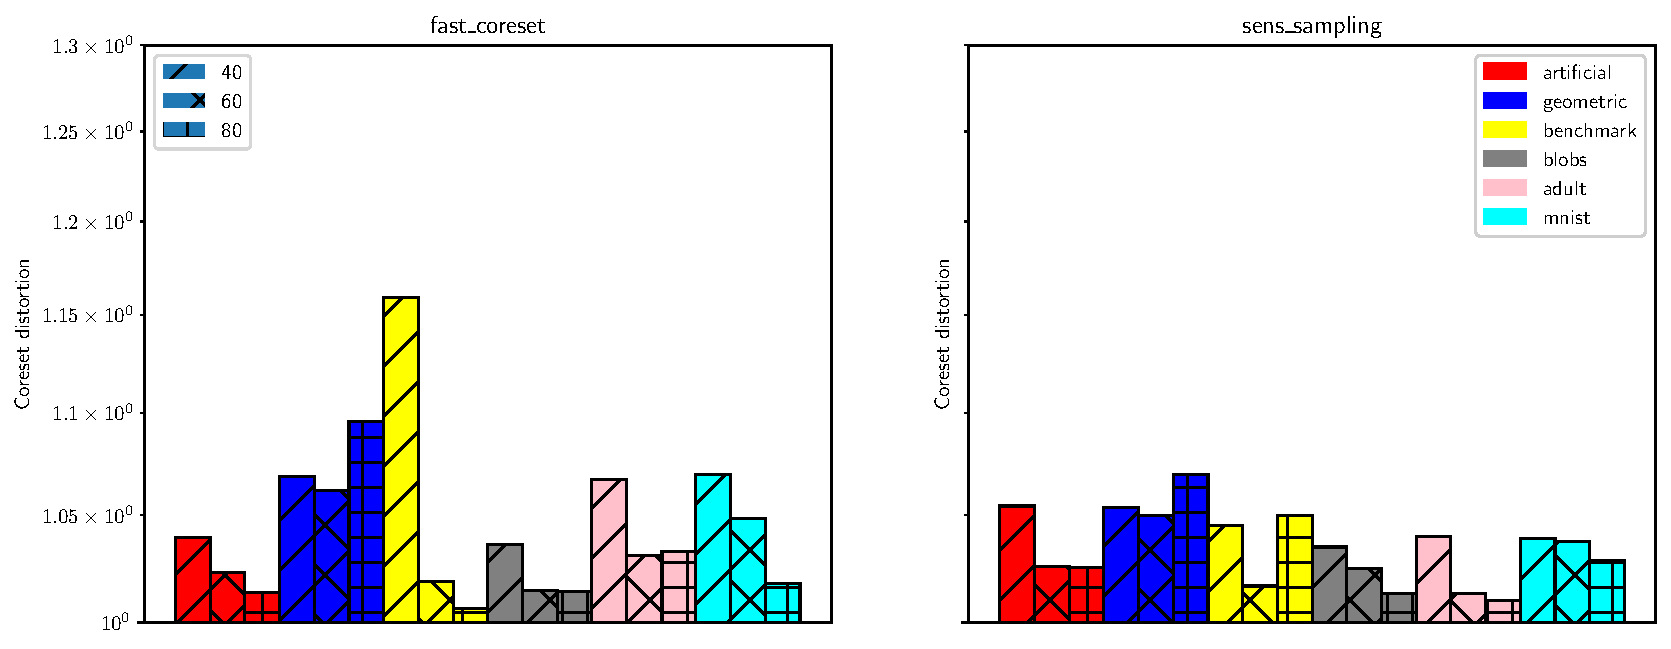
\includegraphics[width=.95\linewidth]{images/1/coreset_distortion-m_scalar_for_sens_sampling.pdf} \\

    \rotatebox[origin=l]{90}{\bf \;\;\quad\quad\quad\quad\quad\quad\quad$k$-Means} &
    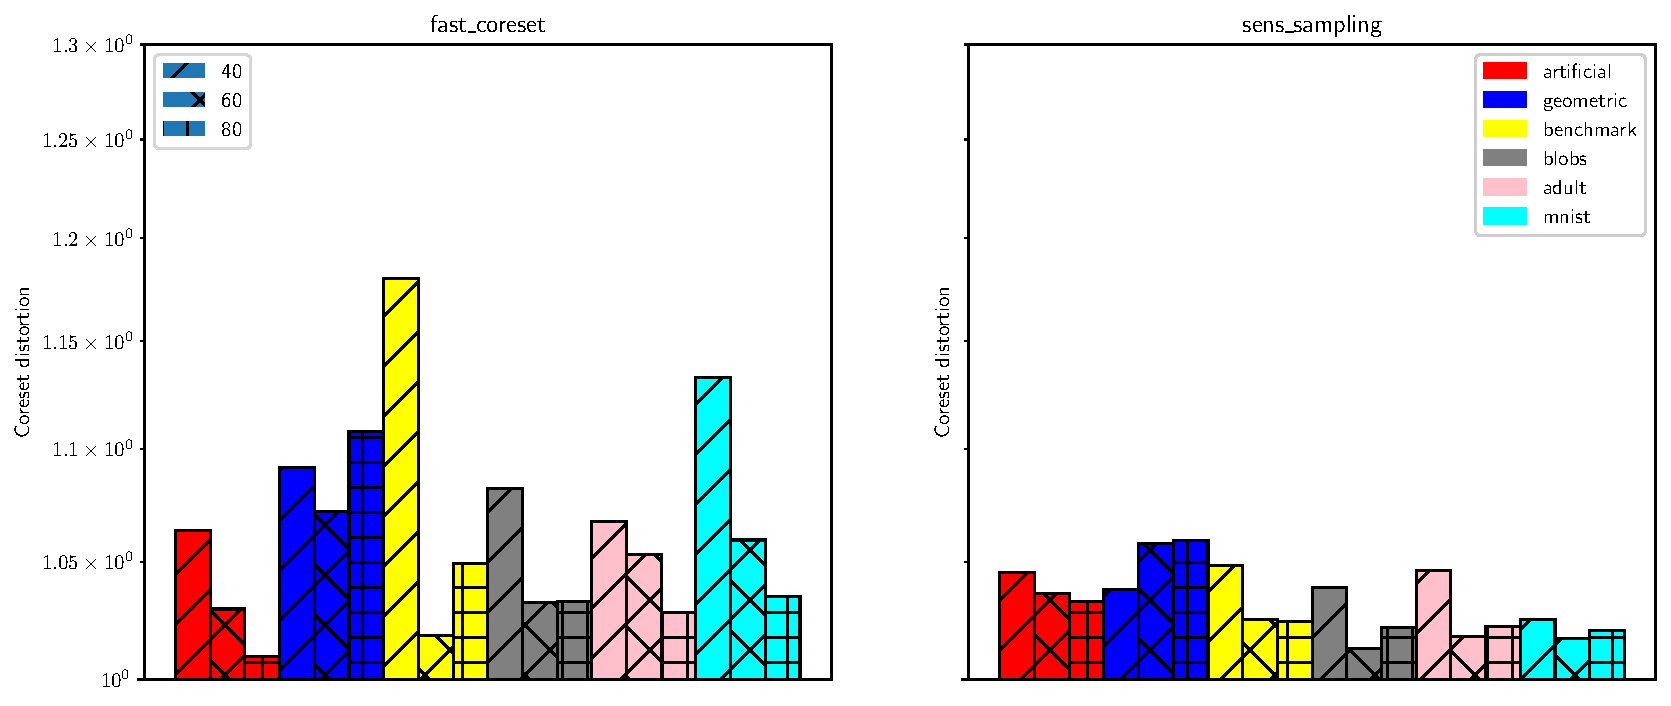
\includegraphics[width=.95\linewidth]{images/2/coreset_distortion-m_scalar_for_sens_sampling.pdf}
\end{tabular}
\caption{The effect of the coreset size on the distortion metric for sensitivity sampling approaches.
We point out that all distortion values are well below $\varepsilon = 0.2$.
Thus, for sufficient coreset sizes, there does not seem to be a meaningful difference between using Fast-Kmeans++ vs. regular Kmeans++.}
\end{figure*}

\begin{figure*}
    \centering
    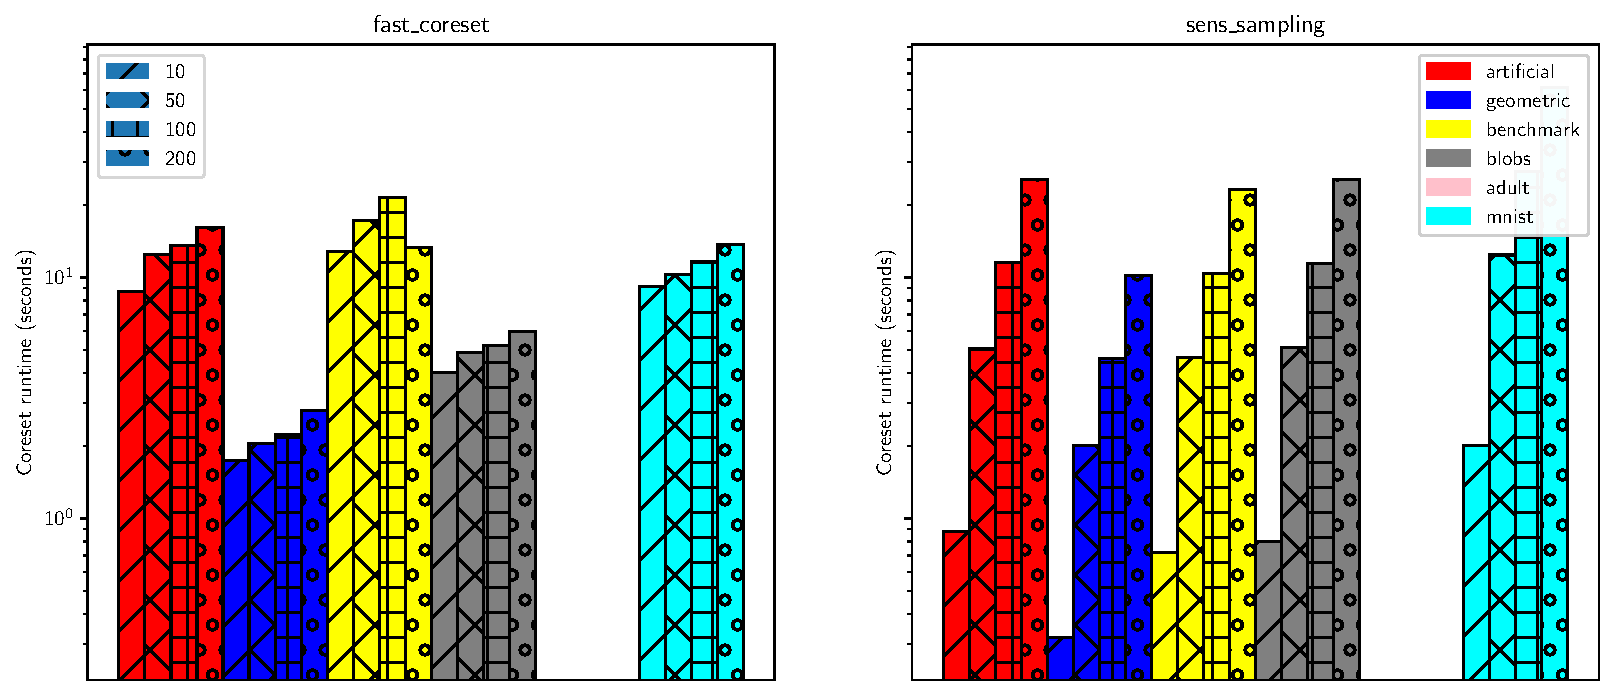
\includegraphics[width=.95\linewidth]{images/2/coreset_runtime-Effect_of_k_for_sens_sampling.pdf}
    \caption{
        The effect of $k$ on the coreset algorithm runtime. We see that traditional sensitivity sampling grows linearly with $k$ while Fast-Kmeans++ grows
        logarithmically.
    }
    \label{fig:k_on_runtime}
\end{figure*}

